

\chapter{弱拓扑和弱*拓扑}



\vspace{-2 em}
\section{Hilbert 空间的定义与基本性质}

% --- 新增过渡 ---
在研究了赋范线性空间和 Banach 空间之后，我们希望引入更丰富的几何结构.
在一般的赋范空间中，我们只有“长度”（范数）和“距离”的概念，却无法衡量向量之间的“夹角”.
为了恢复我们在欧氏几何中熟悉的夹角与正交性，我们引入了内积的概念，这便自然引出了 Hilbert 空间的理论.
% --- 新增过渡结束 ---

\begin{definition}[内积]\index{n@内积}
    设 $X$ 是 $\mb{K} = \mb{R}$ 或 $\mb{C}$ 上的向量空间，$X$ 上的\colorbf{内积}是函数 $\langle \cdot, \cdot \rangle: X \times X \to \mb{K}$，满足：
    \begin{enumerate}
        \item[(i)] $\langle \lambda x + \mu z, y \rangle = \lambda \langle x, y \rangle + \mu \langle z, y \rangle, \forall\, \lambda, \mu \in \mb{K}, x, y, z \in X$.
        \item[(ii)] $\langle x, y \rangle = \overline{\langle y, x \rangle}, \forall\, x, y \in X$.
        \item[(iii)] $\langle x, x \rangle \geqq 0, \forall\, x \neq 0$.
    \end{enumerate}
\end{definition}

由 (i) 可推出关于第二个变量的共轭线性：$\langle x, \lambda y + \mu z \rangle = \bar{\lambda} \langle x, y \rangle + \bar{\mu} \langle x, z \rangle$.
(i) 称为半双线性，(ii) 称为共轭对称性，(iii) 称为正性.\par
可以观察到，若 $\langle \cdot, \cdot \rangle$ 是 $X$ 上的内积，则 $\sqrt{\langle x, x \rangle} =: \|x\|$ 是一个范数.类似于赋范线性空间的概念，可以定义带有内积结构的线性空间.

\begin{definition}[内积空间]\index{n@内积空间}
    设 $X$ 是向量空间，$\langle \cdot, \cdot \rangle$ 是其上的内积，称 $(X, \langle \cdot, \cdot \rangle)$ 为\colorbf{内积空间}.
\end{definition}

由上述观察，内积空间自然是赋范空间.对于由内积诱导出的范数，其一次齐次性和非退化性显然，但三角不等式不是平凡的结果，它依赖于 Cauchy-Schwartz 不等式：

\begin{lemma}[Cauchy-Schwartz不等式]\index{c@Cauchy-Schwartz 不等式}
    设$\|\cdot \|$是$\aab{\cdot,\cdot}$诱导的范数，则
    \begin{equation*}
        \aab{x,y} \leq \norm{x}\norm{y} =\sqrt{\aab{x,x}}\sqrt{\aab{y,y}}.
    \end{equation*}
    等号成立当且仅当存在 $\lambda \in \mb{K}$ 使得 $y = \lambda x$.
\end{lemma}
\begin{proof}
    若 $y = 0$，不等式显然成立且等号成立.下设 $y \neq 0$.
    考虑 $Q(t) = \langle x + ty, x + ty \rangle \geqq 0$，其中 $t \in \mb{K}$.
    根据内积的性质将其展开，得
    \[
        Q(t) = \langle x, x \rangle + t \langle y, x \rangle + \bar{t} \langle x, y \rangle + |t|^2 \langle y, y \rangle \geqq 0.
    \]
    取 $t = -\frac{\langle x, y \rangle}{\langle y, y \rangle}$，代入上式得
    \[
        \langle x, x \rangle - \frac{\langle x, y \rangle \langle y, x \rangle}{\langle y, y \rangle} - \frac{\overline{\langle x, y \rangle} \langle x, y \rangle}{\langle y, y \rangle} + \frac{|\langle x, y \rangle|^2}{\langle y, y \rangle^2} \langle y, y \rangle \geqq 0.
    \]
    注意到 $\langle y, x \rangle = \overline{\langle x, y \rangle}$，上式化简为$\|x\|^2 - \frac{|\langle x, y \rangle|^2}{\|y\|^2} \geqq 0.$\par
    移项即可得到 $|\langle x, y \rangle|^2 \leq \|x\|^2 \|y\|^2$，两边开平方即得 Cauchy-Schwartz 不等式.\par
    等号成立当且仅当$Q(t) = 0$，由内积的正性可知 $x + ty = 0$.
\end{proof}


\begin{proof}[三角不等式的证明]
    \begin{align*}
        \|x + y\|^2 &= \langle x + y, x + y \rangle \\[-3pt]
        &= \langle x, x \rangle + \langle y, x \rangle + \langle x, y \rangle + \langle y, y \rangle \\[-3pt]
        &= \|x\|^2 + \|y\|^2 + 2\Re \langle x, y \rangle.
    \end{align*}
    由于 $|\text{Re} \langle x, y \rangle| \leq |\langle x, y \rangle| \leq \|x\| \|y\|$，
    故 $\|x + y\|^2 \leq \|x\|^2 + \|y\|^2 + 2\|x\| \|y\| = (\|x\| + \|y\|)^2$.
    对两边开根号得三角不等式.
\end{proof}

% --- 新增过渡 ---
既然每个内积空间自然是一个赋范空间，一个自然的反向问题是：什么样的赋范空间可以由内积诱导出来？下述定理给出了完全的几何刻画：
% --- 新增过渡结束 ---

\begin{theorem}[平行四边形法则]\index{p@平行四边形法则}
    设 $(X, \|\cdot\|)$ 是赋范线性空间，则存在 $X$ 上的内积 $\langle \cdot, \cdot \rangle$，使得 $\|x\| = \sqrt{\langle x, x \rangle}$ 当且仅当
    \[
        2\|x\|^2 + 2\|y\|^2 = \|x + y\|^2 + \|x - y\|^2.
    \]
\end{theorem}

% --- 新增过渡 ---
我们将上述条件称为平行四边形法则，其几何意义是：平行四边形的对角线平方和等于四边平方和.当一个范数满足平行四边形法则时，它一定能诱导出内积.那么具体的内积构造公式是什么？这正是接下来的极化恒等式所回答的问题.
% --- 新增过渡结束 ---

\begin{proposition}[极化恒等式]\index{j@极化恒等式}
    设 $(X, \|\cdot\|)$ 是赋范线性空间 使得 $\|\cdot\|$ 来源于内积，则
    \[
        \langle x, y \rangle =
        \begin{cases}
            \frac{1}{4} (\|x + y\|^2 - \|x - y\|^2), & \qif*\mb{K} = \mb{R} \\[7pt]
            \frac{1}{4} (\|x + y\|^2 - \|x - y\|^2 + \iu\|x + \iu y\|^2 - \iu \|x - \iu y\|^2), &\qif* \mb{K} = \mb{C}
        \end{cases}
    \]
\end{proposition}

上述等式与 $x, y$ 的对称性息息相关.

% --- 新增过渡 ---
有了内积之后，为了保证分析中极限运算的良好性质，我们同样需要空间的完备性.正如赋范空间加上完备性构成了 Banach 空间，内积空间加上完备性便构成了我们接下来研究的核心对象——Hilbert 空间.
% --- 新增过渡结束 ---

\begin{definition}[Hilbert 空间]\index{H@Hilbert 空间}
    设 $X$ 是内积空间，若内积诱导出的范数是完备的，则称 $X$ 是 \colorbf{Hilbert 空间}.
\end{definition}

由定义，一切 Banach 空间上的性质/定理对 Hilbert 空间均成立，但由于有极化恒等式，Hilbert 空间应具有更好的性质，其一是定义正交，从而有勾股定理等.但在研究正交之前，我们先来看一些 Hilbert 空间的例子.

\begin{instance}[Hilbert空间的例子]
    \begin{enumerate}
        \item[(0)] $\mb{R}^d, \langle x, y \rangle = \sum_{i=1}^d x_i y_i$；$\mb{C}^d, \langle x, y \rangle = \sum_{i=1}^d x_i \bar{y}_i$.
        \item[(1)] $\ell^2, \langle \{a_n\}, \{b_n\} \rangle = \sum_{n=1}^\infty a_n \bar{b}_n$.
        \item[(2)] $L^2([0,1]), \langle f, g \rangle = \int_0^1 f \bar{g} \d x$.
        \item[(3)] Hilbert 空间的一个闭子空间是 Hilbert 空间.
        \item[(4)] 设$\mb{D} = \{z \in \mb{C} : |z| < 1\}$，定义Bergman 空间为\index{B@Bergman 空间}
        \begin{equation*}
            \mathcal{A}^2(\mb{D}) = \{f \in L^2(\mb{D}, \mb{C}) : f \text{ 是全纯的}\}
        \end{equation*}
        它一个是 Hilbert 空间.\par
        使用 Cauchy 积分公式及 Morera 定理可以证明上述空间是 $L^2(\mb{D}, \mb{C})$ 的闭子空间.
        \item[(5)] 考虑$W^{1,2}((0,1))$，我们通过其中的元素所满足的性质定义该空间.\par
        定义 $u \in W^{1,2}((0,1)) \iff u \in L^2((0,1))$ 且 $\exists\, v \in L^2((0,1)), A \in \mb{R}$，使得 $u(x) = A + \int_0^x v(y) \d y \aew x \in (0,1)$.\par
        它是一个 Sobolev 空间且为 Hilbert 空间.\index{S@Sobolev 空间}\par
        类似地，可以定义$W^{p,2}((0,1))$，它们均是Hilbert空间.
    \end{enumerate}
\end{instance}

\begin{note}
    $W^{1,2}((0,1))$可以嵌入$C([0,1])$，即其中的函数在某种程度上都是连续的.\par
    事实上，取 $u \in W^{1,2}$，$\forall\, x, \tilde{x} \in (0,1)$，
    \[
        |u(x) - u(\tilde{x})| = \left| \int_{\tilde{x}}^x v(y) \d y \right| \leq \|v\|_{L^2} \cdot \|1_{[\tilde{x}, x]}\|_{L^2} = \|v\|_{L^2} \sqrt{|x - \tilde{x}|}.
    \]
    因此
    \[
        \sup_{x \neq \tilde{x} \in (0,1)} \frac{|u(x) - u(\tilde{x})|}{\sqrt{|x - \tilde{x}|}} \leq \|v\|_{L^2} < \infty.
    \]
    其中，左式为 Hölder 半范数 $[u]_{C^{0, \frac{1}{2}}}$，因此 $W^{1,2}((0,1))$ 具有绝对连续性（介于连续与可导之间）.\par
    但由于 $W^{1,2}$ 由等价类定义，更准确地说，上述结论应为 $\forall\, u \in W^{1,2}$，$\exists\, u^* \in W^{1,2}$，使得 $u = u^* \aew$ 且 $u^* \in C([0,1])$，称 $u^*$ 约为 $u$ 的\colorbf{精细表示}.
\end{note}

% --- 新增过渡 ---
进入 Hilbert 空间后，内积的存在使得我们能够严格定义向量之间的“正交”（垂直）关系.这是 Hilbert 空间几何特征的基础，也是它优于一般 Banach 空间的核心所在.
% --- 新增过渡结束 ---

\begin{definition}[正交]\index{z@正交}
    设 $(X, \langle \cdot, \cdot \rangle)$ 是内积空间，称 $x, y \in X$ 是\colorbf{正交}的，当且仅当 $\langle x, y \rangle = 0$，记作 $x \perp y$.\par
    称 $S \subset X, x \in X$ \colorbf{正交}，当且仅当 $\forall\, y \in S, x \perp y$，记作 $x \perp S$.\par
    称 $S, \tilde{S} \subset X$ \colorbf{正交}，当且仅当 $\forall\, x \in S, y \in \tilde{S}, x \perp y$，记作 $S \perp \tilde{S}$.
\end{definition}

\begin{definition}[正交补空间]\index{z@正交补空间}
    设 $X$ 是内积空间，$S \subset X$，定义 $S$ 的\colorbf{正交补空间}为
    \[
        S^\perp := \{x \in X : x \perp S\}.
    \]
\end{definition}

一个观察是 $S^\perp$ 是 $X$ 的闭子空间.\par
设 $x_n \in S^\perp$，$x_n \to y \in X$.则 $\forall\, z \in S$，$\langle y, z \rangle = \lim_{n \to \infty} \langle x_n, z \rangle = 0 \implies y \in S^\perp$.

\begin{note}
    正交补空间有两个重要的性质：$S \subset S^{\perp\perp}$，$\overline{\spann(S)}^\perp = S^\perp$.
\end{note}

% --- 新增过渡 ---
正交的概念为我们解决最佳逼近问题提供了强有力的几何工具.在三维解析几何中，我们知道点到平面的最短距离是由垂线段实现的.在一般的 Hilbert 空间中，只要子集是闭且凸的，这一几何直观依然成立，这便是极为重要的最近点投影定理.
% --- 新增过渡结束 ---

\begin{theorem}[最近点投影]\index{z@最近点投影}
    设 $\mcal{H}$ 为 Hilbert 空间，$K$ 是 $\mcal{H}$ 的非空闭凸子集.则$\forall\, x \in \mcal{H}$，$\exists ! \,y \in K$ 使得 $\|x - y\| = \dist(x, K)$.\par
    特别地，若 $Y \leq \mcal{H}$ 是闭子空间，则 $\forall\, x \in \mcal{H}$，$\exists ! y\,\in Y$ 使得 $x - y \perp Y$.
\end{theorem}
\begin{proof}
    设 $\{y_n\} \subset K$ 是最小化序列，即
    \[
        \|x - y_n\| \searrow \inf \{\|x - z\| : z \in K\} \equiv \dist(x, K) = \delta.
    \]
    考虑平行四边形法则：
    \begin{align*}
        &\quad2\left\| \frac{x - y_n}{2} \right\|^2 + 2\left\| \frac{x - y_m}{2} \right\|^2 = \left\| \frac{2x - y_n - y_m}{2} \right\|^2 + \left\| \frac{y_n - y_m}{2} \right\| ^2, \\
        &\Rightarrow \left\| x - \frac{y_n + y_m}{2} \right\|^2 + \frac{1}{4} \|y_n - y_m\|^2 = \frac{1}{2} (\|x - y_n\|^2 + \|x - y_m\|^2).
    \end{align*}

    当 $n, m \to \infty$ 时，$ \|x - y_n\| \to \delta, \|x - y_m\| \to \delta$.\par
    由于$S$是凸的，$\frac{y_n+y_m}{2}\in S$，故$\norm{x - \frac{y_n + y_m}{2}} \geqq \delta$.\par
    从而 $\|y_n - y_m\| \to 0$.因此 $\{y_n\}$ 是 Cauchy 列.\par
    由 $K$ 是闭的，$y_n \to y \in K$，此时 $\|x - y\| = \delta$.\par
    下证唯一性：设 $y, \tilde{y}$ 均使其最小，通过同样的计算可得
    \begin{equation*}
        \left\| x - \frac{y + \tilde{y}}{2} \right\|^2 + \frac{1}{4} \|y - \tilde{y}\|^2 = \frac{1}{2} (\|x - y\|^2 + \|x - \tilde{y}\|^2).
    \end{equation*}
    此时，$\norm{x-\frac{y+\tilde{y}}{2}}\geqq \delta,\norm{x-y}=\norm{x-\tilde{y}}=\delta$，故
    $\|y-\tilde{y}\|=0\Rrightarrow = \tilde{y}$.\par
    若 $Y$ 是闭子空间，需证$x - y \in Y^\perp$.\par
    由于$\|x-y\|$最小，为其添加围绕，则$\forall\, \tilde{y} \in Y, t \in \mb{R}$，
    \begin{equation*}
        \|x - y\|^2 \leq \|x - y + t\tilde{y}\|^2 = \|x - y\|^2 + 2t\Re \langle x - y, \tilde{y} \rangle + t^2\|\tilde{y}\|^2.
    \end{equation*}
    即$\forall\, t \in \mb{R}$，$t^2\|\tilde{y}\|^2 + 2t\text{Re} \langle x - y, \tilde{y} \rangle \geqq 0$
    $\implies \langle x - y, \tilde{y} \rangle = 0, \forall\, \tilde{y} \in Y$.
\end{proof}


\begin{corollary}
    Hilbert 空间的任一闭子空间均可补.
\end{corollary}

% --- 新增过渡 ---
借助于正交投影，我们希望像在线性代数中那样，找到空间的一组“相互垂直”的基，从而用坐标的形式来简洁地表示任意向量.在无限维情形下，这引导我们定义标准正交基，并由此推广经典的勾股定理.
% --- 新增过渡结束 ---

\section{正交基与 Riesz 表示定理}

\begin{definition}[标准正交集]\index{b@标准正交集}
    设 $\mcal{H}$ 为 Hilbert 空间，称 $S \subset \mcal{H}$ 为\colorbf{标准正交集}当且仅当 $\forall\, x \in S, \|x\| = 1$，且满足$\forall\, x \neq y \in S, \langle x, y \rangle = 0$.
\end{definition}
\begin{definition}[标准正交基]\index{b@标准正交基}
    一个标准正交集 $S$ 被称为\colorbf{标准正交基}当且仅当满足以下任一等价条件：
    \begin{enumerate}
        \item[(i)] 最大的包含 $S$ 的闭子空间是 $\mcal{H}$.
        \item[(ii)] $\overline{\spann(S)} = \mcal{H}$.
        \item[(iii)] $\forall\, x \in \mcal{H}$，$\exists\, \alpha_j \in \mb{K}, s_j \in S$，使得 $\sum_{j=1}^n \alpha_j s_j \to x$，当 $n \to \infty$.
    \end{enumerate}
\end{definition}

需要注意的是，若 $\dim \mcal{H} = \infty$，一个标准正交基不是 Hamel 基.其原因在于 (iii) 的操作已经使其带有拓扑属性.\par
类似有限维的情形，使用 Zorn 引理可以证明 $\mcal{H}$ 一定有标准正交基.\par
在 Hilbert 空间中，标准正交基的存在使得我们能够将任意向量表示为该基的线性组合，并且这种表示是唯一的.这便是勾股定理的核心内容.

\begin{theorem}[勾股定理]\index{g@勾股定理}
    给定任意 $x \in \mcal{H}$ 和有限标准正交集 $S = \{x_1, x_2, \dots, x_n\}$，则
    \[
        \|x\|^2 = \sum_{i=1}^n |\langle x, x_i \rangle|^2 + \left\| x - \sum_{i=1}^n \langle x, x_i \rangle x_i \right\|^2.
    \]
\end{theorem}

\begin{proof}
    \allowdisplaybreaks
    \begin{align*}
        & \quad\left\| x - \sum_{j=1}^n \langle x, x_j \rangle x_j \right\|^2 = \left\langle x - \sum_{j=1}^n \langle x, x_j \rangle x_j, x - \sum_{k=1}^n \langle x, x_k \rangle x_k \right\rangle \\
        &= \|x\|^2 - \left\langle \sum_{j=1}^n \langle x, x_j \rangle x_j, x \right\rangle - \left\langle x, \sum_{k=1}^n \langle x, x_k \rangle x_k \right\rangle + \left\langle \sum_{j=1}^n \langle x, x_j \rangle x_j, \sum_{k=1}^n \langle x, x_k \rangle x_k \right\rangle \\
        &\xlongequal{\langle x_j, x_k \rangle = \delta_{jk}} \|x\|^2 - \sum_{j=1}^n \langle x, x_j \rangle \langle x_j, x \rangle - \sum_{k=1}^n \overline{\langle x, x_k \rangle} \langle x, x_k \rangle + \sum_{j=1}^n \langle x, x_j \rangle \overline{\langle x, x_j \rangle} \\
        &= \|x\|^2 - \sum_{j=1}^n |\langle x, x_j \rangle|^2 - \sum_{k=1}^n |\langle x, x_k \rangle|^2 + \sum_{j=1}^n |\langle x, x_j \rangle|^2 \\
        &= \|x\|^2 - \sum_{j=1}^n |\langle x, x_j \rangle|^2. 
    \end{align*}
    移项后即得勾股定理.
\end{proof}

由于勾股定理仅对有限的标准正交集成立，因此当$\mcal{H}$是无限维的，上述等式无法成立，但可以将上述等式尾项去除，构成一个重要的不等式.

\begin{corollary}[Bessel 不等式]\index{B@Bessel 不等式}
    若 $\dim \mcal{H} = \infty$，$S = \{x_n\}_1^\infty$ 为标准正交集，则
    \[
        \|x\|^2 \geqq \sum_{i=1}^\infty |\langle x, x_i \rangle|^2.
    \]
\end{corollary}

上述不等式取等当且仅当 $\norm{x - \sum_{i=1}^n \langle x, x_i \rangle x_i}\to 0,n \to \infty$，即 $x = \sum_{i=1}^\infty \langle x, x_i \rangle x_i$，这恰好就是标准正交基的定义之一.因此，若 $S$ 是标准正交基，则上述不等式取等.
\begin{corollary}[Parseval 等式]\index{P@Parseval 等式}
    若 $S = \{x_n\}$ 是 $\mcal{H}$ 的标准正交基，则
    \[
        \|x\|^2 = \sum_{i=1}^\infty |\langle x, x_i \rangle|^2.
    \]
\end{corollary}

\begin{instance}
    考虑 
    \begin{equation*}
    C(\mb{T}) = \{f \in C([0,1], \mb{C}) : f(0) = f(1)\},
    \end{equation*}
    并赋予它 $L^2$ 内积以及对应的$L^2$ 范数.\par
    由于 $C(\mb{T})$ 在 $L^2$ 范数下是不完备的，我们定义 $L^2(\mb{T}) := \overline{C(\mb{T})}^{L^2}$ 为其在 $L^2$ 范数下的完备化闭包，即将所有 $L^2$ 柯西列的极限包含进来.\par
    所得到的 $L^2(\mb{T})$ 正是环面上的复值平方可积的可测函数空间，它保留了内积结构并变得完备，因而是 Hilbert 空间.\par
    $L^2(\mb{T})$ 的一个标准正交基是 $\{e_n\}_{n \in \mb{Z}}$，其中 $e_n(x) := \eu^{2\pi \iu n x}$.\par
    则
    \begin{align*}
        f &= \sum_{n \in \mb{Z}} \langle f, e_n \rangle e_n \in L^2(\mb{T}) \\[-3pt]
        &= \sum_{n \in \mb{Z}} \left( \int_0^1 f \bar{e}_n \d x \right) e_n.
    \end{align*}
    \allowdisplaybreaks
    \begin{align*}
        f(x) &= \sum_{n \in \mb{Z}} \left( \int_0^1 f(y) \eu^{-2\pi\iu n y} \d y \right) \eu^{2\pi\iu n x} \\[-2pt]
        &= \sum_{n \in \mb{Z}} \hat{f}(n) \eu^{2\pi\iu n x} \\[-2pt]
        &= \sum_{n \in \mb{Z}} \int_0^1 f(y) \eu^{2\pi\iu n (x-y)} \d y
    \end{align*}
    
    由 Parseval 等式，$\|f\|_{L^2}^2 = \sum_{n \in \mb{Z}} |\langle f, e_n \rangle|^2$，
    即 $\|f\|_{L^2}^2 = \sum_{n=-\infty}^\infty |\hat{f}(n)|^2 = \|\{\hat{f}(n)\}_{n \in \mb{Z}}\|_{\ell^2}^2$.
    
    因此，若考虑映射 \begin{align*}
        \mcal{F}:L^2(\mb{T}) &\to \ell^2(\mb{Z}), \\[-5pt]
        f &\mapsto \{\hat{f}(n)\}_{n \in \mb{Z}}.
    \end{align*}
    则$\mcal{F}$是 $L^2 \to \ell^2$ 的等距同构.\par
    更一般的，若脱离具体的空间，若存在可数标准正交基 $\{e_n\}$，映射 $\mcal{F}: \mcal{H} \to \ell^2, x \mapsto \{\langle x, e_n \rangle\}_{n \in \mb{N}}$ 是一个等距同构.
\end{instance}
上述例子说明任意具有可数标准正交基的 Hilbert 空间都与 $\ell^2$ 等距同构.从而引发我们思考能否对Hilbert空间作分类.\par
\textbf{断言}：一个可分 Hilbert 空间必有可数标准正交基.
\begin{corollary}
    设 $\mcal{H}$ 是 Hilbert 空间，若$\mcal{H}$可分，则$\mcal{H} \cong \ell^2$.
\end{corollary}

对一般的$L^2$空间 $L^2(\Omega, \d\mu)$，一个可选的标准正交基是Laplace算子的特征向量$\{\psi_n\}$，即满足 $-\Delta \psi_n = \lambda_n \psi_n, 0 \leq \lambda_1 \leq \dots \nearrow \infty$.

% --- 新增过渡 ---
在掌握了 Hilbert 空间的基本几何结构之后，我们自然想考察它的对偶空间.Hilbert 空间由于其极好的对称性和正交投影性质，其上的所有连续线性泛函都可以由内积完全表示.
% --- 新增过渡结束 ---

\begin{theorem}[Hilbert 空间的 Riesz 表示]\index{R@Riesz 表示定理}
    $\forall\, f \in \mcal{H}^* = \mcal{B}(\mcal{H}; \mb{K})$，$\exists !\, x \in \mcal{H}$，使得 $f(y) = \langle y, x \rangle, \forall\, y \in \mcal{H}$，即 $f \hat{=} \langle \cdot, x \rangle$.\par
    进一步，$\|f\|_{\mcal{H}^*} = \|x\|_{\mcal{H}}$.\par
\end{theorem}

\begin{proof}
    若 $f = 0$，则 $x = 0$.\par
    假设 $f \neq 0$，设 $Z = \ker f \leq \mcal{H}$，则 $\mcal{H} = Z \oplus Z^\perp$.\par
    为找到 $x \in \mcal{H}$ 表示 $f$，任取 $w \in Z^\perp \setminus \{0\}$，
    则 $\forall\, y \in \mcal{H}$，$y - \frac{f(y)}{f(w)} w \in Z$.\par
    $\implies \ab(y - \frac{f(y)}{f(w)} w) \perp w$，即 $\left\langle y - \frac{f(y)}{f(w)} w, w \right\rangle = 0$，得 $f(y) = \frac{f(w)}{\|w\|^2} \langle y, w \rangle$.\par
    即 $\forall\, y \in \mcal{H}, f(y) = \langle y, x \rangle$，其中 $x = \frac{\overline{f(w)}}{\|w\|^2} w$.\par
    下证唯一性：若 $f \in \mcal{H}^*$ 有两个表示 $x, \tilde{x} \in \mcal{H}$,
    \begin{equation*}
    f(y) = \langle y, x \rangle = \langle y, \tilde{x} \rangle, \forall\, y \in \mcal{H}.
    \end{equation*}
    则$\langle y, x - \tilde{x} \rangle = 0, \forall\, y \in \mcal{H}$，故 $x - \tilde{x} \in \mcal{H}^\perp = \{0\}$.\par
    最后验证等距性：由 Cauchy-Schwartz 不等式，$\forall\, y \in \mcal{H}$，
    \begin{equation*}
        |f(y)| = |\langle y, x \rangle| \leq \|x\| \|y\|
    \end{equation*}
    $\implies \|f\| \leq \|x\|$.上述不等式等号在 $y = x$ 时取到，由此 $\|f\| = \|x\|$.
\end{proof}

\begin{corollary}
    Hilbert 空间 $\mcal{H}$ 与其对偶空间 $\mcal{H}^*$ 是等距同构的.
\end{corollary}
这一结论与典型的Banach空间的性质形成了鲜明的对比.对于一般的Banach空间，其对偶空间往往比原空间大得多.


\section{弱收敛}
% --- 新增过渡 ---
借助于 Riesz 表示定理建立的泛函与元素的对应关系，我们可以在 Hilbert 空间（或更一般的赋范空间）上探究一种比范数收敛更弱的收敛性.这在处理无法获得强收敛的情形下非常有用.
% --- 新增过渡结束 ---

\begin{definition}[弱收敛]\index{r@弱收敛}
    设 $X$ 是赋范线性空间，$\{x_n\} \subset X$，若
    \begin{equation*}
        f(x_n) \to f(x), \forall\, f \in X^*,
    \end{equation*}
    则称 $x_n$ \colorbf{弱收敛}到 $x$，记作 $x_n \rightharpoonup x$.
\end{definition}
回顾强收敛的定义，$x_n \to x$ 当且仅当 $\|x_n - x\| \to 0$，这意味着 \begin{equation*}
    \forall\, f \in X^*,|f(x_n - x)| \leq \|f\| \|x_n - x\| \to 0,
\end{equation*}
从而 $f(x_n) \to f(x)$.这表明强收敛蕴含弱收敛，但反之不然.因此，弱收敛是一种比强收敛更宽松的收敛概念.\par

\begin{note}
    由 Banach-Steinhaus 定理，若 $x_n \rightharpoonup x$，$\sup \|x_n\| < \infty$.\par
    考虑典范嵌入 $J_X : X \hookrightarrow X^{**}, x \mapsto J_X(x)(f) = f(x)$.\par
    $\{x_n\}$ 弱收敛意味着 $J_X(x_n)$ 点态收敛.
\end{note}

\begin{proposition}
    设 $X$ 是赋范线性空间，$\{x_n\} \subset X, x_n \rightharpoonup x \in X$当且仅当$J_X(x_n) \to J_X(x)$.
\end{proposition}

% --- 新增过渡 ---
除了弱收敛，在对偶空间中我们还可以引入一种更弱的收敛性，即弱*收敛.这在处理泛函序列时尤为重要.
% --- 新增过渡结束 ---

\begin{definition}[弱*收敛]\index{r@弱*收敛}
    设 $X$ 是 Banach 空间，$\{f_n\} \subset X^*$.若
    \begin{equation*}
        f_n(x) \to f(x),\forall\, x\in X
    \end{equation*}
    则称 $f_n$ \colorbf{弱*收敛}到 $f$，记作 $f_n \weakstar f$.
\end{definition}

\begin{attention}
    比较弱收敛与弱*收敛，注意弱*收敛并为要求在进一步取对偶空间的元素作试验，而是在原空间的元素上作试验.因此，弱*收敛比弱收敛更弱.以下面三个情形为例
    \begin{itemize}
        \item 对于 $x_n \in X$，$x_n \rightharpoonup x \iff f(x_n) \to f(x), \forall\, f \in X^*$.
        \item 对于 $f_n \in X^*$，$f_n \rightharpoonup f \iff \Phi(f_n) \to \Phi(f), \forall\, \Phi \in X^{**}$.
        \item 对于 $f_n \in X^*$，$f_n \weakstar f \iff f_n(x) \to f(x), \forall\, x \in X$.
    \end{itemize}
    由于可以通过典范嵌入 $J: X \hookrightarrow X^{**}$ 将 $X$ 视为 $X^{**}$ 的子空间，我们有：若 $f_n \rightharpoonup f$，则 $f_n \weakstar f$.反之一般不成立.
\end{attention}

% --- 新增过渡 ---
上面我们给出了弱收敛的抽象定义，它的直觉非常朴素：我们不要求序列在范数意义下逼近极限，而只要求在每一个连续线性泛函作用下逼近.换句话说，在某种意义上，"弱"通常带有"试验"的含义——弱收敛即是在泛函（试验函数）作用下收敛.与此类似的还有弱解、弱导数等概念，这种思想在分析中随处可见.
% --- 新增过渡结束 ---

\begin{instance}
    对于 $\ell^p (1 < p < \infty)$，其对偶空间 $(\ell^p)^* \cong \ell^{p'}$，其中 $\frac{1}{p} + \frac{1}{p'} = 1$.事实上，上述同构可以由下述映射刻画：
    \begin{align*}
        \Phi : (\ell^p)^* &\to \ell^{p'} \\[-5pt]
        T &\mapsto a = \{a_n\}
    \end{align*}
    使得$\forall\, b = \{b_n\} \in \ell^p$，$Tb = \sum_{n=1}^\infty a_n b_n$.
    可以证明 $\ell^p (1 < p < \infty)$ 是自反空间. \par
    考虑 $\ell^p$ 中的标准单位向量 $\{e_n\}_{n \in \mb{N}} \subset \ell^p$，其中 $(e_n)_j = \delta_{nj}$.则 $\{e_n\}$ 无强收敛子列，但 $e_n \rightharpoonup 0$.
    事实上，任取 $T \in (\ell^p)^*$，设 $\Phi(T) = a \in \ell^{p'}$，则：
    \begin{equation*}
        T e_n = \sum_{k=1}^\infty a_k (e_n)_k = a_n \to 0 \quad \ab(\text{由于 } \sum_{n=1}^\infty |a_n|^{p'} < \infty)
    \end{equation*}
    故 $\{e_n\}$ 在 $\ell^p (1 < p < \infty)$ 中弱收敛到 $0$.
\end{instance}

% --- 新增过渡 ---
上面我们看到，对于 $1 < p < \infty$，$\ell^p$ 中的单位向量序列弱收敛但不强收敛.这一现象依赖于 $\ell^p$ 的对偶空间 $\ell^{p'}$ 中元素的坐标趋于零这一事实.然而，当 $p = 1$ 时情况截然不同.
% --- 新增过渡结束 ---

\begin{attention}
    在 $\ell^1$ 中，$e_n \not\rightharpoonup 0$.\par
    由于 $(\ell^1)^* = \ell^\infty$，我们可以取 $s = (1, -1, 1, -1, \dots) \in \ell^\infty$.此时对 $e_n$ 作用可得 $(-1)^{n+1}$.因此 $\exists\, T = \Phi^{-1}(s) \in (\ell^1)^*$，使得 $T e_n$ 不收敛.
\end{attention}

% --- 新增过渡 ---
事实上，$\ell^1$ 中的情形远比上面这个反例所揭示的更深刻：不仅是标准正交基不弱收敛于零，整个 $\ell^1$ 空间中弱收敛与强收敛是等价的.
% --- 新增过渡结束 ---

\begin{theorem}[Schur 定理]\index{S@Schur 定理}
    在 $\ell^1$ 空间中，序列的弱收敛当且仅当其强收敛.
\end{theorem}
\begin{proof}
    \fbox{$\Leftarrow$} 显然.\par
    \fbox{$\Rightarrow$} 假设在 $\ell^1$ 中 $x_n \rightharpoonup 0$ 但 $x_n \not\to 0$.\par
    则 $\exists\, \varepsilon > 0$，有子列$\{y_n\} \subset \{x_n\}$，使得
    \begin{equation*}
        \norm{y_n} \geq \varepsilon > 0.\tag{1}
    \end{equation*}
    记 $y_n = \{y_{n,k}\}_{k \in \mb{N}}$.\par
    由 $y_n \rightharpoonup 0$，考虑在第 $k$ 个坐标上的投影泛函，有对于固定的 $k$，$y_{n,k} \to 0$ ($n \to \infty$).从而对每个固定的$p \in \mb{N}$，当$n\to \infty$时，$\sum_{i=1}^p|y_{n,k}|\to 0$.\par
    因此，$\forall\, p\in\mb{N},\exists\, n = n(p, \varepsilon)$，使得
    \begin{equation*}
        \sum_{k=1}^p |y_{n(p),k}| < \frac{\varepsilon}{4}. \tag{2}
    \end{equation*}
    并且由(1)，必定 $\exists\, q > p$，使得
    \begin{equation*}
        \sum_{k=p+1}^q |y_{n,k}| > \frac{3\varepsilon}{4}, \quad \sum_{k=q+1}^\infty |y_{n,k}| < \frac{\varepsilon}{4}.
    \end{equation*}
    将上述的$p$和对应的$n$提取为序列$\{p_i\},\{n_i=n(p_i,\varepsilon)\}$，使得 
    \begin{equation*}
        \sum_{1 \leq k \leq p_i} |y_{n_i, k}| < \frac{\varepsilon}{4}, \quad \sum_{p_i + 1 \leq k \leq p_{i+1}} |y_{n_i, k}| > \frac{3\varepsilon}{4}, \quad \sum_{k \geq p_{i+1} + 1} |y_{n_i, k}| < \frac{\varepsilon}{4}.
    \end{equation*}
    定义符号序列 $s \in \ell^\infty \cong (\ell^1)^*$ 如下：
    \begin{equation*}
        s_k = \begin{cases}
            0, & \qif k <p_i,\\
            \operatorname{sgn}(y_{n_i, k}), & \qif p_i \leq k \leq p_{i+1},\\
        \end{cases}
    \end{equation*}
    则作用在 $y_{n_i}$ 上得到：
    \begin{align*}
        \sum_{k=1}^\infty s_k y_{n_i, k} &=\sum_{k=1}^\infty\operatorname{sgn}(y_{n_i, k}) \chi_{[p_i, p_{i+1}]}(k)y_{n_i, k}\\
        &\xlongequal{\operatorname{sgn}(x)x=|x|}\sum_{k=1}^\infty |y_{n_i, k}| \chi_{[p_i, p_{i+1}]}(k)\\
        &\geq \frac{3\varepsilon}{4} - \frac{\varepsilon}{4} - \frac{\varepsilon}{4} = \frac{\varepsilon}{4} > 0.
    \end{align*}
    这与 $x_n \rightharpoonup 0$矛盾.
\end{proof}

上述定理证明的关键在于构造了一个两边取值小但中心取值大的序列，我们通常称之为「驼峰」，上述证明的技巧被称为驼峰移动.更进一步我们可以证明，

\begin{corollary}
    任意 $\ell^1$ 空间的无限维闭子空间的对偶空间不可分.
\end{corollary}

现在考虑性质更好的Hilbert空间.若 $\mcal{H}$ 是可分 Hilbert 空间且其标准正交基为 $\{e_n\}$，可以验证 $e_n \rightharpoonup 0$.\par
以 $L^2(\mb{T})$ 为例，$\forall \varphi \in L^2(\mb{T})$，由 Riemann-Lebesgue 引理，有：
\begin{equation*}
    \int_0^1 \sin(2\pi nx)\varphi(x) \d x \to 0, \quad \int_0^1 \cos(2\pi nx)\varphi(x) \d x \to 0.
\end{equation*}
从中可以发现，弱收敛但不强收敛的典型例子是\bluebf{振荡函数}.另一类常见的例子是\bluebf{分布函数}，例如 $f_n(x) = \frac{n}{2} \chi_{(-\frac{1}{n}, \frac{1}{n})}$.它在 $L^1$ 上一致有界，但在 $L^1$ 中不收敛.其极限从直观上仅在 $x=0$ 处取到无穷大，在 $L^1$ 中无意义，但在弱*拓扑下有意义.


\begin{definition}[Dirac delta 测度]\index{D@Dirac delta 测度}
    定义$\delta_0 \in [C_0^\infty(\mb{R})]^*$，使得 $\delta_0(f) = f(0), \forall f \in C_0^\infty(\mb{R})$.称其为 \colorbf{Dirac delta 测度}.
\end{definition}

回归正题设 $\mcal{H}$ 是 Hilbert 空间，$\{e_n\}$ 是其标准正交基.我们要说明 $e_n \rightharpoonup 0$.\par
设 $T$ 是 $\mcal{H}^*$ 中的任意泛函，由 Riesz 表示定理，$\exists !\, a \in \mcal{H}$，使得 $T e_n = \aab{e_n, a}$.\par
由 Parseval 等式，$\sum_{n=1}^\infty |\aab{e_n, a}|^2 \leq \norm{a}_{\mcal{H}}^2 < \infty$.\par
故当 $n \to \infty$ 时，$|T e_n| = |\aab{e_n, a}| \to 0$.这即证明了 $e_n \rightharpoonup 0$.\par



\section{弱拓扑与弱*拓扑}

我们知道强收敛是由范数诱导的拓扑下的收敛.这引发我们思考弱收敛和弱*收敛能否由某种结构来刻画.这就引出了$X$ 上的弱拓扑和 $X^*$ 上的弱*拓扑.

\begin{definition}[弱拓扑]\index{r@弱拓扑}
    设 $X$ 是赋范线性空间，$X$ 上的\colorbf{弱拓扑}，记作$w$，由具有如下形式的拓扑基生成：
    \begin{equation*}
        O = \{x \in X : |f_i(x - x_0)| < \varepsilon, \forall\,1 \leq i \leq n\}
    \end{equation*}
    其中 $\varepsilon > 0, x_0 \in X, n \in \mb{N}$ 且 $f_1, \dots, f_n \in X^*$.
\end{definition}

\begin{definition}[弱*拓扑]\index{r@弱*拓扑}
    设 $X$ 是赋范线性空间，$X^*$ 上的\colorbf{弱*拓扑}，记作$w^*$，由具有如下形式的拓扑基生成：
    \begin{equation*}
        O = \{f \in X^* : |(f - g)(x_i)| < \varepsilon, \forall\,1 \leq i \leq n\}
    \end{equation*}
    其中 $n \in \mb{N}, \varepsilon > 0, g \in X^*$ 且 $x_1, \dots, x_n \in X$.
\end{definition}

从拓扑视角来看，弱拓扑和弱*拓扑分别是使得所有 $X^*$ 中的元素或 $X$ 中的元素连续的最弱拓扑.因此，弱拓扑和弱*拓扑正是由足够多的线性泛函（或足够多的点）生成的，这种"足够多"恰好由 Hahn-Banach 定理保证，从而使这两个拓扑都是 Hausdorff 的.

\begin{proposition}
    $(X, w)$ 和 $(X^*, w^*)$ 都是 Hausdorff 空间.
\end{proposition}
\begin{proof}
    给定 $x \neq y \in X$，由 Hahn-Banach 定理，$\exists f \in X^*, \alpha \in \mb{R}$，使得 $f(x) > \alpha > f(y)$.\par
    则 $x \in \{v \in X : f(v) > \alpha\}$，且 $y \in \{v \in X : f(v) < \alpha\}$.\par
    这两个集合均为弱拓扑下开集，故 $x, y$被开集分离，从而 $(X, w)$ 是 Hausdorff 的.\par
    对 $(X^*, w^*)$ 的证明类似.
\end{proof}

% --- 新增过渡 ---
以下几条命题总结了弱拓扑与弱*拓扑的基本性质，包括闭集刻画、序列收敛与拓扑收敛的等价性等.这些性质虽然叙述简单，但在后续的自反性判别和紧性讨论中将被反复使用.
% --- 新增过渡结束 ---

\begin{proposition}
    $A \subset X$ 弱紧，即 $A\subset (X, w)$紧 $\iff J_X(A)$ 在 $(X^{**}, w^*)$ 中弱*收敛.
\end{proposition}

\begin{proposition}
    在 $X^*$ 中，$f_n \stackrel{*}{\rightharpoonup} f \iff f_n \to f$ 逐点收敛.
\end{proposition}

我们之前提及到一致收敛是在sup范数下的收敛.但从上述命题中可以看出，逐点收敛可以看作弱*收敛，但弱*收敛不可度量，自然逐点收敛不可能是某个范数的收敛.因而，一致收敛应当比逐点收敛强得多.\par

下一个命题回答了我们引入弱拓扑和弱*拓扑的初衷：它们正是为了刻画弱收敛和弱*收敛而设计的.因此，在这两个拓扑下，序列的极限与我们之前定义的弱收敛和弱*收敛完全一致.

\begin{proposition}
    对 $f, f_1, f_2, \dots \in X^*$，$f_n \to f\qin (X^*, w^*)$ ，当且仅当 $f_n(x) \to f(x), \forall x \in X$.\par
    对 $x, x_1, x_2, \dots \in X$，$x_n \to x\qin (X, w)$，当且仅当 $f(x_n) \to f(x), \forall f \in X^*$.
\end{proposition}
\begin{proof}
    仅证第一部分.\fbox{$\Rightarrow$}显然.\par
    \fbox{$\Leftarrow$}假设 $f_n \to f$ 逐点收敛.任取 $f$ 的 弱*开邻域，记作 $O$.\par
    则 $\exists\,\varepsilon > 0, x_1, \dots, x_m \in X$，使得 $f \in \tilde{O} = \bigcap_{i=1}^m \{g \in X^* : |(g-f)(x_i)| < \varepsilon\} \subset O$.\par
    由 $f_n \to f$ 逐点收敛，$\exists\, N \in \mb{N},\st\forall\, n > N$，$|f_n(x_i) - f(x_i)| < \varepsilon,\forall\,i \in \{1, \dots, m\}$.\par
    因此当 $n > N$ 时，$f_n \in \tilde{O} \subset O$.\par
    这就说明在$f$的任意弱*开邻域与$\{f_n\}$相交，从而$(X^*, w^*)$ 中 $f_n \to f$.
\end{proof}

弱拓扑和弱*拓扑确实是较为抽象的概念，但在有限维空间中，所有 Hausdorff 向量空间拓扑彼此等价，因此弱拓扑、弱*拓扑与范数拓扑一致.
% --- 新增过渡结束 ---

\begin{proposition}
    若 $\dim X < \infty$，则 $X$ 上的弱拓扑和范数拓扑相容；$X^*$ 上的弱*拓扑和范数拓扑相容.
\end{proposition}
\begin{proof}
    设 $O \subset X^*$ 是开集，验证$O$ 是弱*开的.\par
    任取 $f_0 \in O$，则 $\exists \varepsilon > 0$，使得 $f_0 + \varepsilon B_{X^*} \subset O$.\par
    由于 $\dim X < \infty$，设 $\{e_1, \dots, e_n\}$ 是 $X$ 的基.定义 $\interleave f \interleave = \max_{1 \leq i \leq n} |f(e_i)|$.\par
    在有限维空间上，$\interleave \cdot \interleave$ 与范数 $\norm{\cdot}$ 等价.因此，$\exists \delta > 0$，使得 $\interleave f \interleave < \delta \implies \norm{f} < \varepsilon$.\par
    可以构造弱*邻域：
    \begin{equation*}
        \tilde{O} = \bigcap_{i=1}^d \{f \in X^* : |(f- f_0)(e_i)| < \delta\}
    \end{equation*}
    则 $\tilde{O} \subset f_0 + \varepsilon B_{X^*} \subset O$.进而 $O$ 是弱*开集.\par
    对于弱拓扑，利用
    \begin{equation*}
        (X,w)\cong (X^{**}, w^*)=(X^**, \norm{\cdot})\cong (X,\norm{\cdot})\qedhere 
    \end{equation*}
\end{proof}

\begin{attention}
    若 $\dim X = \infty$，弱拓扑严格比范数拓扑粗糙.\par
    事实上，$0$ 附近的基本的 弱开集形式为
    \begin{equation*}
            O = \bigcap_{i=1}^n \{x \in X : |f_i(x)| < \varepsilon\},\qq{for some} f_1,\cdots,f_n\in X^*, \varepsilon > 0.
    \end{equation*}
    观察到 $\bigcap_{i=1}^n \ker f_i \subset O$，而这在无限维空间中是一个余维度有限的无限维子空间.\par
    从而 $O$ 在范数下无界，不可能被任何范数拓扑下的开球所包含.
\end{attention}

% --- 新增过渡 ---
下面这个命题给出了二次对偶空间中的哪些元素真正来自于原空间.
% --- 新增过渡结束 ---

\begin{proposition}
    设 $X$ 是 Banach 空间，$F \in X^{**}$.若 $F$ 在 $X^*$ 上弱*连续，则 $\exists\, x \in X$，使得 $F = J_X(x)$.
\end{proposition}
\begin{proof}
    设 $F$ 是弱*连续的，则 $\exists \varepsilon > 0$ 以及 $x_1, \dots, x_n \in X$，使得
    \begin{equation*}
        |F(f)| \leq 1, \quad \forall f \in U_\varepsilon = \bigcap_{i=1}^n \{g \in X^* : |g(x_i)| < \varepsilon\}.
    \end{equation*}

    考虑$\mcal{N} = \bigcap_{i=1}^n \{g \in X^* : g(x_i) = 0\} = \bigcap_{i=1}^n \ker J_X(x_i)$.\par
    显然 $0 \in N \subset U_\varepsilon$，且 $N$ 是一个子空间.\par
    由于对 $\forall f \in N \subset U_\varepsilon$ 均有 $|F(f)| \leq 1$，而 $\mcal{N}$ 是子空间，这迫使 $F(f) = 0, \forall f \in \mcal{N}$.\par
    由代数中关于线性泛函的引理，$F$ 必然是 $J_X(x_1), \dots, J_X(x_n)$ 的线性组合：
    \begin{equation*}
        F = \sum_{i=1}^n \alpha_i J_X(x_i) = J_X\left(\sum_{i=1}^n \alpha_i x_i\right).
    \end{equation*}
    取 $x = \sum_{i=1}^n \alpha_i x_i \in X$ 即得.
\end{proof}

% --- 新增过渡 ---
由之前的讨论，我们知道任意的弱开集都是范数意义下的开集.那么反之，任意范数意义下的闭集都是弱闭集，这意味着存在不是弱闭的闭集.下一个引理讨论了在添加什么条件后，闭集也是弱闭的.
% --- 新增过渡结束 ---

\begin{lemma}[Mazur 引理][lem:Mazur引理]\index{M@Mazur 引理}
    Banach 空间的每个凸闭子集都是弱闭的.
\end{lemma}
\begin{proof}
    设 $C \subset X$ 是闭且凸的.只需证明$X \setminus C$ 是弱开的.\par
    任取 $x_0 \in X \setminus C$.由于 $C$ 闭凸且 $x_0 \notin C$，由Hahn-Banach 定理，\begin{equation*}
        \exists\, f \in X^*, \alpha \in \mb{R},\st f(x_0) > \alpha > \sup_{x \in C} f(x).
    \end{equation*}
    因此 $x_0 \in \{f> \alpha\} \subset X \setminus C$，其中$\{f>\alpha\}$弱开.\par
    故 $X \setminus C$ 是弱开集.
\end{proof}

\begin{definition}[凸包]\index{t@凸包}
    集合 $S$ 的\colorbf{凸包}是最小的包含 $S$ 的凸集，记作 $\operatorname{conv}(S)$.\par
    其闭包为闭凸包，记作 $\overline{\operatorname{conv}}(S) = \operatorname{cl} \ab\{ \sum_{i=1}^n \lambda_i s_i : 0 \leq \lambda_i \leq 1, \sum \lambda_i = 1, s_i \in S \}$.
\end{definition}
\begin{note}
    由 Mazur 引理可知，对于 $\overline{\operatorname{conv}}(S)$，它上面的弱拓扑和范数拓扑诱导的闭集（从而拓扑结构在某种意义上）是紧密相关的，其弱闭包与范数闭包相同.
\end{note}

% --- 新增过渡 ---
Mazur 引理关于凸集的结果还有一个极为实用的推论：弱收敛序列可以借助凸组合"提升"为强收敛.
% --- 新增过渡结束 ---

\begin{corollary}
    若 $x_n \rightharpoonup x$，则存在 $\{x_n\}$ 的凸组合强收敛到 $x$.
\end{corollary}

% --- 新增过渡 ---
我们最后讨论无穷维对偶空间中单位球面的弱*稠密性.在有限维空间中，单位球面是紧的且不含原点，自然不可能弱*逼近原点.但在无限维空间中，原点属于单位球面的弱*闭包.
% --- 新增过渡结束 ---

\begin{theorem}
    若 $\dim X = \infty$，则 $0 \in \overline{\mb{S}_{X}}^{w}$，且 $\overline{\mb{S}_{X}}^{w} = \overline{\mb{B}_X}$.
\end{theorem}
\begin{proof}
    需要证明 $0$ 的任意弱开邻域均与$\mb{S}_{X}$ 相交.\par
    由于无穷维空间中任意的基本弱邻域必定包含一个无限维的子空间，而任何无限维子空间必然会穿过单位球面.故结论成立.
\end{proof}

上述定理在弱*拓扑中也有类似的结论.

\begin{theorem}[Josefson-Nissenzweig 定理]\index{J@Josefson-Nissenzweig 定理}
    设 $X$ 是无穷维 Banach 空间，则存在序列 $\{f_n\} \subset S_{X^*}$，使得 $f_n \weakstar 0$.
\end{theorem}



\section{Banach-Alaoglu 定理}

% --- 新增过渡 ---
Josefson-Nissenzweig 定理揭示了无穷维对偶球面的弱*收敛现象，这本质上源于弱*拓扑的不可度量性.对于通常不可度量的拓扑空间，其拓扑性质需借助"网"这一工具来刻画.下面我们从网的基本概念开始，逐步建立一般乘积空间的紧性理论（Tychonoff 定理），并利用它给出 Banach-Alaoglu 定理的完整证明.
% --- 新增过渡结束 ---

\begin{definition}[指标集]\index{z@指标集}
    集合 $I$ 是\colorbf{指标集}当且仅当它上面有偏序.
\end{definition}

\begin{definition}[网]\index{w@网}
    设 $X$ 是非空集合，$X$ 中的\colorbf{网}是映射
    \begin{align*}
    N: I &\to X,\\[-3pt]
    \alpha &\mapsto x_\alpha.
    \end{align*}
\end{definition}

\begin{definition}[子网]\index{w@网!z@子网}
    设 $\{x_\alpha\}_{\alpha\in I}$ 是网，则 $\{x_{s(\beta)}\}_{\beta\in J}\subset \{x_\alpha\}_{\alpha\in I}$ 是\colorbf{子网}若其满足
    \begin{enumerate}
        \item[(i)] $J$ 是指标集.
        \item[(ii)] $s: J\to I$ 是映射，满足 $\forall\, \alpha_0\in I, \exists\, \beta_0\in J,\ \st \beta_0\leq \beta \Rightarrow \alpha_0\leq s(\beta)$.
    \end{enumerate}
\end{definition}

直观而言，子网是子序列概念在一般拓扑空间中的自然推广.对于网来说，定义中的 (ii)实际要求提取出来的网「趋于无穷」：不论在原指标集 $I$ 中选定多靠后的界限 $\alpha_0$，映射 $s$ 总能在新指标集 $J$ 中找到一个时刻 $\beta_0$，只要过了这个时刻（即 $\beta_0 \leq \beta$），映射出的原指标 $s(\beta)$ 都会不可逆地跨过前面的界限 $\alpha_0$.此外，有别于普通情况下的子序列，子网的指标提取映射 $s$ 并不需要是单射，也无需严格保序.

\begin{definition}[网的收敛]\index{w@网!w@网的收敛}
    设 $\{x_\alpha\}_{\alpha\in I}$ 是网，称 $\{x_\alpha\}_{\alpha\in I}$ \colorbf{收敛}到 $x$ 当且仅当对 $x$ 的任意开邻域 $U$，存在 $\alpha_0\in I$，使得 $\forall\, \alpha\geq \alpha_0, x_\alpha\in U$.
\end{definition}

% --- 新增过渡 ---
有了网的收敛概念，我们可以处理任意拓扑空间中的极限.接下来的 Tychonoff 定理是点集拓扑学的基石之一，它断言任意多个紧空间的乘积仍是紧的.
% --- 新增过渡结束 ---

\begin{theorem}[Tychonoff 定理]\index{T@Tychonoff 定理}
    设 $I$ 是任意非空集合，$\forall\, \alpha\in I$，$X_\alpha$ 是紧集，则 $\prod_{\alpha\in I} X_\alpha$ 在乘积拓扑下是紧的.
\end{theorem}

由此我们可以证明以下深刻的结果.无穷维赋范线性空间中的单位球一定不是范数意义下的紧集，但是其对偶空间的单位闭球在弱*拓扑下却是紧的.这就是 Banach-Alaoglu 定理.

\begin{theorem}[Banach-Alaoglu 定理][thm:BA定理]\index{B@Banach-Alaoglu 定理}
    设 $X$ 是 Banach 空间，则 $(\overline{\mb{B}_{X^*}}, w^*)$ 是紧的.
\end{theorem}
\begin{proof}
    考虑 \begin{equation*}
        \{f: \overline{\mb{B}_X}\to [-1,1]\} = \prod_{\overline{\mb{B}_X}} [-1,1],
    \end{equation*}
    由 Tychonoff 定理，$\{f: \overline{\mb{B}_X}\to [-1,1]\}$ 在逐点收敛的拓扑下紧.\par
    定义 $\mcal{F} = \{f|_{\overline{\mb{B}_X}}: f\in \overline{\mb{B}_{X^*}}\} $，那么$\forall f\in \overline{\mb{B}_{X^*}}, x\in \overline{\mb{B}_X},\ |f(x)|\leq \norm{f}\norm{x}\leq 1$.\par
    因此$\mcal{F}\subseteq \prod_{\overline{\mb{B}_X}} [-1,1]$.\par
    注意$f_n \weakstar f$ 就是 $f_n$ 逐点收敛到 $f$.因此可以构造双射
    \begin{align*}
    \Phi: \overline{\mb{B}_{X^*}} &\to \mcal{F}\\[-5pt]
    f &\mapsto f|_{\overline{\mb{B}_X}}
    \end{align*}
    因此$(\overline{\mb{B}_{X^*}}, w^*) \cong (\mcal{F}, \text{逐点收敛的拓扑})$.\par
    由于 $\prod_{\overline{\mb{B}_X}} [-1,1]$ 紧，下证 $(\mcal{F}, \text{ptwise})$闭.\par
    任取网 $\{f_\alpha\}_{\alpha\in I}\subset (\mcal{F}, \text{ptwise})$, $\st f_\alpha \to f_\infty\qin \prod_{\overline{\mb{B}_X}} [-1,1]$.\par
    将 $f_\infty$ 延拓到 $X$ 上为 $F_\infty$:
    \[
    F_\infty(x) := \begin{cases} 0, & \text{if } x=0,\\ \norm{x} f_\infty\ab(\frac{x}{\norm{x}}), & \text{if } x\in X\setminus\{0\}. \end{cases}
    \]
    因为每个$f_\alpha$都线性，故$f_\infty$线性，进而$F_\infty\in X'$.\par
    并且有
    \begin{equation*}
        \norm{F_\infty} = \sup\{|F_\infty(x)|: \norm{x}\leq 1\}
    = \sup\{|f_\infty(x)|: \norm{x}\leq 1\}
    \leq \norm{f_\infty}\leq 1.
    \end{equation*}
    因而 $F_\infty\in \overline{\mb{B}_{X^*}}$，于是 $f_\infty = F_\infty|_{\overline{\mb{B}_X}} \in \mcal{F}$.\par
    故 $\mcal{F}$ 在逐点收敛拓扑下闭，从而紧，即 $(\overline{\mb{B}_{X^*}}, w^*)$ 紧.
\end{proof}
% --- 新增过渡 ---
上述定理证明的核心思路是将对偶单位球嵌入到紧乘积空间 $\prod_{\overline{\mb{B}_X}} [-1,1]$ 中，再利用 Tychonoff 定理验证其像集的闭性.
% --- 新增过渡结束 ---


% --- 新增过渡 ---
Banach-Alaoglu 定理的一个重要应用场景是紧度量空间上的 Radon 测度理论与概率论中弱分布收敛的联系.
% --- 新增过渡结束 ---

设 $K$ 是紧度量空间，则 $[C(K)]^* \cong \mcal{M}(K)$，其中 $\mcal{M}(K)$ 为 $K$ 上 Radon 测度.\par
依据定理，可以显式地写出它们之间的映射：
\begin{align*}
\Phi: \mcal{M}(K) &\to [C(K)]^*\\[-3pt]
\mu &\mapsto \Phi(\mu):\begin{aligned}[t]
    C(K)&\to \mb{K}\\[-3pt]
    f&\mapsto \int_K f \d\mu
\end{aligned} 
\end{align*}
其中$\mcal{M}(K)$ 的范数定义为
\[
\norm{\mu} := \sup\ab\{ \sum_{j=1}^\infty |\mu(E_j)|: E_j\subset K,\ \bigsqcup_{j=1}^\infty E_j = K \}.
\]

设 $\{P_j\}$ 是紧集 $K$ 上的概率测度，则 $\forall j,\ \norm{P_j}\leq 1$，故 $\{P_j\}\subset \overline{\mb{B}_{\mcal{M}(K)}} = \overline{\mb{B}_{[C(K)]^*}}$.\par
由 Banach-Alaoglu 定理，$\exists\ \{P_{j_k}\}\subset \{P_j\},\ \st P_{j_k} \weakstar \mu\in \mcal{M}(K)$.\par
等价地，$\forall f\in C(K)$, $\int_K f \d P_{j_k} \to \int_K f\d\mu,\ j\to\infty$.\par
由此得到了概率中的弱分布收敛.


% --- 新增过渡 ---
Banach-Alaoglu 定理保证了对偶单位球的弱*紧性.在此基础上，一个自然的问题是：弱拓扑和弱*拓扑在通常情况下无法赋予度量，那么弱拓扑或弱*拓扑上的单位球能否在一定条件下可度量化的？下面的定理给出了完整的回答.
% --- 新增过渡结束 ---

\begin{theorem}[可度量化]\index{k@可度量化}
    \begin{enumerate}
        \item[(i)] $(\overline{\mb{B}_{X^*}}, w^*)$ 可度量化 $\iff$ $X$ 可分.
        \item[(ii)] $(\overline{\mb{B}_X}, w)$ 可度量化 $\iff$ $X^*$ 可分.
        \item[(iii)] 若 $X$ 可分，则对任意弱紧集 $C\subset X$，$(C,w)$ 可度量化.
    \end{enumerate}
\end{theorem}

% --- 新增过渡 ---
在进行 (ii) 的 证明之前，我们先插入一个重要的引理——Goldstine 引理，它刻画了 $X$ 在二次对偶中的弱*稠密性，同时也是完成上述证明的关键工具.
% --- 新增过渡结束 ---

\begin{lemma}[Goldstine 引理]\index{G@Goldstine 引理}
    $$\overline{J_X(\mb{B}_X)}^{w^*} = \mb{B}_{X^{**}}.$$
\end{lemma}

\begin{proof}
    \fbox{$\subseteq$} $J_X(\overline{\mb{B}_X})\subseteq \mb{B}_{X^{**}}$ $\xrightarrow{\text{\cref{thm:BA定理}}}$ $\overline{J_X(\mb{B}_X)}^{w^*}\subseteq \overline{\mb{B}_{X^{**}}}^{w^*} = \mb{B}_{X^{**}}$.\par
    \fbox{$=$} 假设 $\exists \xi\in \mb{B}_{X^{**}}\setminus \overline{J_X(\mb{B}_X)}^{w^*}$.\par
    由 Hahn-Banach 定理，$\exists f\in X^*$, $\st \xi(f) > \sup\{\eta(f): \eta\in \overline{J_X(\mb{B}_X)}^{w^*}\}$.\par
    由于 $\xi, \eta$ 的连续性，可使 $f$ 正规化且 $\xi(f)>1$.\par
    但 $\sup\{\eta(f): \eta\in \overline{J_X(\mb{B}_X)}^{w^*}\} = \sup\{f(x_0): x_0\in \overline{\mb{B}_X}\} = \norm{f}$，故
    $f(x_0)=\eta(f)\leq 1$, $\forall \eta\in J_X(\mb{B}_X)$, $\ie \eta=J_X(x_0), x_0\in \mb{B}_X$.\par
    $\Rightarrow \norm{f}\leq 1$, 与 $\xi\in \mb{B}_{X^{**}}$, $\xi(f)>1$ 矛盾.
\end{proof}

\begin{proof}[(ii) 的证明]
    \fbox{$\Leftarrow$} 设 $X^*$ 可分，则存在可数稠密子集 $\{f_n\}_{n=1}^\infty \subset \mb{S}_{X^*}$.\par
    定义 $\rho(x,y) = \sum_{n=1}^\infty \frac{|f_n(x-y)|}{2^n}$, $\forall x,y\in \overline{\mb{B}_X}$.\par
    则 $\rho$ 是 $(\overline{\mb{B}_X}, w)$ 上的度量.\par
    需要验证 $\mathrm{Id}: (\overline{\mb{B}_X}, w)\to (\overline{\mb{B}_X}, \rho)$ 连续.

    \fbox{$\Rightarrow$} 设 $(\overline{\mb{B}_X}, w)$ 可度量化.
\end{proof}





% --- 新增过渡 ---
现在回到可度量化定理 (ii) 的 $\Rightarrow$ 方向.
% --- 新增过渡结束 ---

则 $0\in X$ 有弱拓扑下的可数邻域基 $\{U_n\}_{n\in \mb{N}}$，那么对 $\forall n$, $\exists m_n\in \mb{N}, f_j\in X^*$, 有
\[
U_n = \bigcap_{j=1}^{m_n} \{x\in X: |f_{n_j}(x)|<\varepsilon_n\}.
\]

设 $\mcal{F} = \bigcup_{n=1}^\infty \{f_{n_1},\ldots, f_{n,m_n}\} \subseteq X^*$.\par
断言：$\overline{\spann}\mcal{F} = X^*$.\par
pf: 若不然，$\exists f\in X^*$, $\st \dist(f, \mcal{F})\geq \delta>0$.\par
由 Hahn-Banach 定理，$\exists \xi\in X^{**}$, $\st$
\[
\begin{cases} \xi|_{\overline{\spann}(\mcal{F})} = 0\\ \xi(f)=1,\ \norm{\xi}=\frac{1}{\delta}. \end{cases}
\]

考虑 $V=\{x\in \overline{\mb{B}_X}: |f(x)|<\frac{\delta}{2}\}$，这是 $0$ 的一个弱开邻域，因而包含某些 $U_n$.\par
可以选择 $x_1\in \overline{\mb{B}_X}$ $\st$ $|\xi(f)-J_X(x_1)(f)|<\frac{\delta}{2}$，
且 $|g(x_1)| = |\xi(g)-g(x_1)|<\varepsilon_n,\ \forall g\in \overline{\spann}(\mcal{F})$.\par
因此，$x_1\in U_n\setminus V$，矛盾.\par
进而 $X^*$ 可分.

$\ell^\infty$ 不可分，又 $(\ell^\infty)^* = \ell^1$，因此 $(\overline{\mb{B}_{\ell^1}}, w)$ 不可度量.


\section{Krein-Milman 定理}
% --- 新增过渡 ---
以上讨论了弱拓扑的度量化条件.接下来我们转向凸性理论的核心：Krein-Milman 定理.该定理断言紧凸集可以由其"极点"生成，这是研究凸体结构的基本工具.下面首先给出极点的定义.
% --- 新增过渡结束 ---

\begin{definition}[极点]\index{j@极点}
    设 $X$ 是 Banach 空间，$C\subset X$，称 $x\in C$ 是 $C$ 的\colorbf{极点}，记作 $x\in \operatorname{Ext}(C)$，当且仅当 $x$ 不是 $C$ 中任意线段的中点.
\end{definition}

\begin{theorem}[Krein-Milman 定理]\index{K@Krein-Milman 定理}
    设 $X$ 是 Banach 空间.
    \begin{enumerate}
        \item[(i)] 若 $K\subset X$ 是弱紧且是凸的，则 $K = \overline{\operatorname{conv}}(\operatorname{Ext}(K))$.
        \item[(ii)] 若 $K\subset X^*$ 是弱*紧且凸的，则 $K = \overline{\operatorname{conv}}^{w^*}(\operatorname{Ext}(K))$.
    \end{enumerate}
\end{theorem}

\begin{definition}[支撑流形]\index{z@支撑流形}
    设 $X$ 是 Banach 空间，$K\subset X$ 凸，$H$ 是仿射子空间，则称 $H$ 是 $K$ 的\colorbf{支撑流形}当且仅当
    \[
    \begin{cases}
    H\cap K = \varnothing,\\
    \text{若 } [x,y]\subset K \text{ 在 } H \text{ 中有内点，则 } [x,y]\subset H.
    \end{cases}
    \]
\end{definition}

\begin{figure}[H]
    \centering
    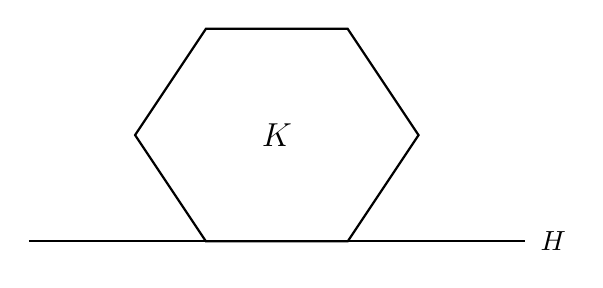
\begin{tikzpicture}[thick, scale=0.9]

    % 1. 绘制水平直线 H
    \draw (-1, 0) -- (6, 0) node[right=2pt] {$H$};

    % 2. 绘制上方的多边形（凸集 K），底边与直线 H 重合
    \draw (1.5, 0) -- (3.5, 0) -- (4.5, 1.5) -- (3.5, 3) -- (1.5, 3) -- (0.5, 1.5) -- cycle; % cycle 用于闭合路径

    % 3. 在多边形中心添加标签 K
    \node at (2.5, 1.5) {\large $K$};

\end{tikzpicture}
    \captionof{figure}{支撑流形}
\end{figure}



% --- 新增过渡 ---
Krein-Milman 定理的证明依赖于以下关键断言：任何闭支撑流形必包含极点.下面先陈述该断言，再给出定理的验证.
% --- 新增过渡结束 ---
\begin{claim*}
    设 $X$ 是 Banach 空间，$K\subset X$ 是弱紧且凸的，若 $H$ 是 $K$ 的闭支撑流形，则 $H\cap \operatorname{Ext}(K)\neq \varnothing$.
\end{claim*}

承认上述断言，可以验证 $K\subseteq \overline{\operatorname{conv}}^w(\operatorname{Ext}(K))$.\par
假设 $\exists c\in K\setminus \widetilde{K}$，其中 $\widetilde{K} = \overline{\operatorname{conv}}^w(\operatorname{Ext}(K))$.\par
由 Hahn-Banach 定理，$\exists f\in X^*$, $\st \alpha = \sup_K f \geq f(c) > \sup_{\widetilde{K}} f$.\par
则 $f^{-1}\{\alpha\} = H$ 是 $K$ 的支撑超平面.\par
那么，由断言，$H$ 包含 $x\in \operatorname{Ext}(K)$，则 $f(x) = \alpha = \sup_K f > \sup_{\widetilde{K}} f$.\par
由于 $f$ 连续，从而弱连续，故 $f(x) = \sup_K f$ 矛盾.

\begin{figure}[H]
\begin{center}
    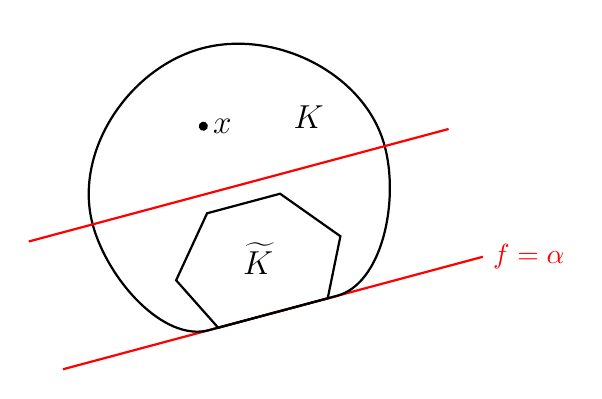
\begin{tikzpicture}[scale=1.2, rotate=15] % 整体旋转15度，还原手绘的倾斜感

    % 1. 绘制底部的支撑超平面 f = \alpha (红色平行线)
    % 设底线在 y = -1 的水平线上。红线比公用底边长。
    \draw[thick, red] (-2.3, -1) -- (2.3, -1) node[right, text=red] {$f=\alpha$};

    % 2. 绘制外部的大凸集 K (极致平滑的新形状)
    % 中心大约在 (0, 0.45)，外围半径约 1.6-1.7
    % 使用全贝塞尔路径实现圆弧和直线的自然平滑过渡，确保在底部与 y = -1 完全公用共线。
    % 通过更柔和的控制点实现极致自然平滑的过渡。
    \draw[thick] (-0.7, -1) -- (0.7, -1) % 公用底边
          .. controls (1.2, -1) and (1.6, -0.2) .. (1.6, 0.4) % 右下平滑过渡，圆弧切点在 (1.6, 0.4)
          .. controls (1.6, 1.2) and (0.8, 1.9) .. (0, 1.9) % 顶部圆弧
          .. controls (-0.8, 1.9) and (-1.6, 1.2) .. (-1.6, 0.4) % 左上圆弧，圆弧切点在 (-1.6, 0.4)
          .. controls (-1.6, -0.2) and (-1.2,-1) .. cycle; % 左下平滑过渡，回到底边
    % 标签在大凸集 K 的主体上
    \node[font=\large] at (0.9, 0.9) {$K$};

    % 3. 绘制内部的小凸集 (对应证明中的 \tilde{K})
    % 凸多边形，底边 (-0.6, -1) -- (0.6, -1) 严格落在 y = -1 的公用边上。
    \draw[thick] (-0.6, -1) -- (0.6, -1) -- (0.9, -0.4) -- (0.4, 0.2) -- (-0.4, 0.2) -- (-0.9, -0.4) -- cycle;
    % 标签在内部小图形上
    \node[font=\large] at (0, -0.4) {$\widetilde{K}$};

    % 4. 绘制中间的分离超平面 (红色平行线)
    % 同一个泛函 f 的等值线，必然与 y = -1 严格平行，通过 y = 0.4
    \draw[thick, red] (-2.3, 0.4) -- (2.3, 0.4);

    % 5. 绘制极点 x (对应证明中的点 c)
    % 确保它位于分离超平面上方，大凸集内部
    \filldraw (-0.2, 1.1) circle (1.2pt);
    \node[right, font=\large] at (-0.2, 1.1) {$x$};

\end{tikzpicture}
    \captionof{figure}{Krein-Milman 定理证明示意图}
\end{center}
\end{figure}


% 下面给出关键断言的完整证明：任何闭支撑流形必包含极点.
% 证明的核心是 Zorn 引理 —— 在全体支撑流形构成的偏序集中取极小元，并证明极小支撑流形与 K 的交是单点集.

\begin{proof}[关键断言的证明]
设 $H$ 是 $K$ 的闭支撑流形.考虑 $H$ 的所有支撑仿射子流形构成的集合族
\begin{equation*}
\mcal{M} = \ab\{\widetilde{H} : \widetilde{H}\subseteq H \text{ 为 }\,K\,\text{ 上支撑仿射流形}\}.
\end{equation*}
该族在 $\supseteq$ 下构成偏序集.\par
设 $\{H_\alpha\}_{\alpha\in I}\subseteq \mcal{M}$ 是 $\mcal{M}$ 中的链（全序集）.\par
令 $\displaystyle H_\infty = \bigcap_{\alpha\in I} H_\alpha$，下证 $H_\infty\in\mcal{M}$.\par
首先，由于每个 $H_\alpha\cap K\neq\varnothing$，且 $\{H_\alpha\cap K\}_{\alpha\in I}$ 是弱紧集 $K$ 中满足 $\supseteq$ 序关系的链，由弱紧性得 $\bigcap_{\alpha\in I} (H_\alpha\cap K)\neq\varnothing$，故 $H_\infty\cap K\neq\varnothing$.\par
其次，验证支撑流形条件.设 $[x,y]\subseteq K$ 在 $H_\infty$ 中有内点.则 $\forall\,\alpha\in I$，$(x,y)\cap H_\alpha\neq\varnothing$，由 $H_\alpha$ 是支撑流形知 $[x,y]\subseteq H_\alpha$，$\forall\,\alpha\in I$，故 $[x,y]\subseteq H_\infty$.\par
综上，$H_\infty\in\mcal{M}$，且它是该链的一个上界.由 Zorn 引理，$\mcal{M}$ 存在极小元，记为 $M_0$.\par
下证 $M_0\cap K = \{x_0\}$，则 $x_0\in \operatorname{Ext}(K)$.\par
反证，假设 $\exists\, x\neq y\in M_0\cap K$.由于 $x\neq y$，可取 $f\in X^*$，$\st f(x)\neq f(y)$.\par
由于 $M_0\cap K$是弱紧集的闭集，故也为弱紧集，因而$f$ 在其上达到最大值，即
\begin{equation*}
\exists\, k\in M_0\cap K,\st f(k) = \sup_{z\in M_0\cap K} f(z) \equiv \alpha.
\end{equation*}
则 $f^{-1}\{\alpha\}$ 是 $K$ 的支撑超平面，且 $k\in M_0\cap K\cap f^{-1}\{\alpha\}$.\par
考虑 $\widetilde{M} := M_0\cap f^{-1}\{\alpha\}$.由支撑流形与支撑超平面的交仍为支撑流形，$\widetilde{M}$ 仍是 $K$ 的支撑仿射流形，故 $\widetilde{M}\in\mcal{M}$.\par
由于 $f(x)\neq f(y)$，$x,y$ 不可能同时属于 $f^{-1}\{\alpha\}$，因此 $x,y$ 中至少其一不在 $\widetilde{M}$ 中.\par
故 $\widetilde{M}\subsetneq M_0$，这与 $M_0$ 的极小性矛盾.\par
因此 $M_0\cap K$ 为单点集，从而 $H\cap \operatorname{Ext}(K)\neq\varnothing$.
\end{proof}

% --- 新增过渡 ---
由上述关键断言立即得出以下两个有用的观察.
% --- 新增过渡结束 ---

\begin{corollary}[]
设 $K\subseteq X$ 是弱紧且凸的，则 $K$ 存在支撑超平面.\par
进一步，若 $H\subseteq X$ 是 $K$ 的支撑流形且 $H\cap K = \{x\}$，则 $x\in \operatorname{Ext}(K)$.
\end{corollary}
\begin{proof}
任取 $f\in X^*$，由于 $K$ 弱紧，$f$ 在 $K$ 上达到最大值，记 $\alpha = \sup_K f$.\par
则 $H = f^{-1}\{\alpha\}$ 为 $K$ 的支撑超平面.\par
若支撑流形 $H$ 满足 $H\cap K = \{x\}$，由关键断言，$x$ 必为极点，故 $x\in \operatorname{Ext}(K)$.
\end{proof}


